\documentclass[10pt,letterpaper,final,twoside,notitlepage]{article}
\usepackage[margin=.5in]{geometry} % 1/2 inch margins on all pages
\usepackage[utf8]{inputenc} % Define the input encoding
\usepackage[USenglish]{babel} % Define language used
\usepackage{amsmath,amsfonts,amssymb}
\usepackage{amsthm} % Gives us plain, definition, and remark to use in \theoremstyle{style}
\usepackage{mathtools} % Allow for text and math in align* environment.
\usepackage{thmtools}
\usepackage{thm-restate}
\usepackage{graphicx}

\usepackage[
backend=biber,
style=alphabetic,
citestyle=authoryear]{biblatex} % Must include citation somewhere in document to print bibliography
\usepackage{hyperref} % Generate hyperlinks to referenced items
\usepackage[nottoc]{tocbibind} % Prints the Reference/Bibliography in TOC as well
\usepackage[noabbrev,nameinlink]{cleveref} % Fancy cross-references in the document everywhere
\usepackage{nameref} % Can make references by name to places
\usepackage{caption} % Allows for greater control over captions in figure, algorithm, table, etc. environments
\usepackage{subcaption} % Allows for multiple figures in one Figure environment
\usepackage[binary-units=true]{siunitx} % Gives us ways to typeset units for stuff
\usepackage{csquotes} % Context-sensitive quotation facilities
\usepackage{enumitem} % Provides [noitemsep, nolistsep] for more compact lists
\usepackage{chngcntr} % Allows us to tamper with the counter a little more
\usepackage{empheq} % Allow boxing of equations in special math environments
\usepackage[x11names]{xcolor} % Gives access to coloring text in environments or just text, MUST be before tikz
\usepackage{tcolorbox} % Allows us to create boxes of various types for examples
\usepackage{tikz} % Allows us to create TikZ and PGF Pictures
\usepackage{ctable} % Greater control over tables and how they look
\usepackage{diagbox} % Allow us to have shared diagonal cells in tables
\usepackage{multirow} % Allow us to have a single cell in a table span multiple rows
\usepackage{titling} % Put document information throughout the document programmatically
\usepackage[linesnumbered,ruled,vlined]{algorithm2e} % Allows us to write algorithms in a nice style.

\counterwithin{figure}{section}
\counterwithin{table}{section}
\counterwithin{equation}{section}
\counterwithin{algocf}{section}
\crefname{algocf}{algorithm}{algorithms}
\Crefname{algocf}{Algorithm}{Algorithms}
\setcounter{secnumdepth}{4}
\setcounter{tocdepth}{4} % Include \paragraph in toc
\crefname{paragraph}{paragraph}{paragraphs}
\Crefname{paragraph}{Paragraph}{Paragraphs}

% Create a theorem environment
\theoremstyle{plain}
\newtheorem{theorem}{Theorem}[section]
% Create a numbered theorem-like environment for lemmas
\newtheorem{lemma}{Lemma}[theorem]

% Create a definition environment
\theoremstyle{definition}
\newtheorem{definition}{Defn}
\newtheorem{corollary}{Corollary}[section]
% \begin{definition}[Term] \label{def:}
%   Make sure the term is emphasized with \emph{term}.
%   This ensures that if \emph is changed, it shows up everywhere
% \end{definition}

% Create a numbered remark environment numbered based on definition
% NOTE: This version of remark MUST go inside a definition environment
\theoremstyle{remark}
\newtheorem{remark}{Remark}[definition]
%\counterwithin{definition}{subsection} % Uncomment to have definitions use section.subsection numbering

% Create an unnumbered remark environment for general use
% NOTE: This version of remark has NO restrictions on placement
\newtheorem*{remark*}{Remark}

% Create a special list that handles properties. It can be broken and restarted
\newlist{propertylist}{enumerate}{1} % {Name}{Template}{Max Depth}
% [newlistname, LevelsToApplyTo]{formatting options}
\setlist[propertylist, 1]{label=\textbf{(\roman*)}, ref=\textbf{(\roman*)}, noitemsep, nolistsep}
\crefname{propertylisti}{property}{properties}
\Crefname{propertylisti}{Property}{Properties}

% Create a special list that handles enumerate starting with lower letters. Breakable/Restartable.
\newlist{boldalphlist}{enumerate}{1} % {Name}{Template}{Max Depth}
% [newlistname, LevelsToApplyTo]{formatting options}
\setlist[boldalphlist, 1]{label=\textbf{(\alph*)}, ref=\alph*, noitemsep, nolistsep} % Set options

\newlist{nocrefenumerate}{enumerate}{1} % {Name}{Template}{Max Depth}
% [newlistname, LevelsToApplyTo]{formatting options}
\setlist[nocrefenumerate, 1]{label=(\arabic*), ref=(\arabic*), noitemsep, nolistsep}

% Create a list that allows for deeper nesting of numbers. By default enumerate only allows depth=4.
\newlist{nestednums}{enumerate}{6}
% [newlistname, LevelsToApplyTo]{formatting options}
\setlist[nestednums]{noitemsep, label*=\arabic*.}

\tcbuselibrary{breakable} % Allow tcolorboxes to be broken across pages
% Create a tcolorbox for examples
% /begin{example}[extra name]{NAME}
% Create a tcolorbox for examples
% Argument #1 is optional, given by [], that is the textbook's problem number
% Argument #2 is mandatory, given by {}, that is the title for the example
% Avoid putting special characters, (), [], {}, ",", etc. in the title.
\newtcolorbox[auto counter,
number within=section,
number format=\arabic,
crefname={example}{examples}, % Define reference format for cref (No Capitals)
Crefname={Example}{Examples}, % Reference format for cleveref (With Capitals)
]{example}[2][]{ % The [2][] Means the first argument is optional
  width=\textwidth,
  title={Example \thetcbcounter: #2. #1}, % Parentheses and commas are not well supported
  fonttitle=\bfseries,
  label={ex:#2},
  nameref=#2,
  colbacktitle=white!100!black,
  coltitle=black!100!white,
  colback=white!100!black,
  upperbox=visible,
  lowerbox=visible,
  sharp corners=all,
  breakable
}

% Create a tcolorbox for general use
\newtcolorbox[% auto counter,
% number within=section,
% number format=\arabic,
% crefname={example}{examples}, % Define reference format for cref (No Capitals)
% Crefname={Example}{Examples}, % Reference format for cleveref (With Capitals)
]{blackbox}{
  width=\textwidth,
  % title={},
  fonttitle=\bfseries,
  % label={},
  % nameref=,
  colbacktitle=white!100!black,
  coltitle=black!100!white,
  colback=white!100!black,
  upperbox=visible,
  lowerbox=visible,
  sharp corners=all
}

% Redefine the 'end of proof' symbol to be a black square, not blank
\renewcommand{\qedsymbol}{$\blacksquare$} % Change proofs to have black square at end

% Common Mathematical Stuff
\newcommand{\Abs}[1]{\ensuremath{\lvert #1 \rvert}}
\newcommand{\DNE}{\ensuremath{\mathrm{DNE}}} % Used when limit of function Does Not Exist

% Complex Numbers functions
\renewcommand{\Re}{\operatorname{Re}} % Redefine to use the command, but not the fraktur version
\renewcommand{\Im}{\operatorname{Im}} % Redefine to use the command, but not the fraktur version
\newcommand{\Real}[1]{\ensuremath{\Re \lbrace #1 \rbrace}}
\newcommand{\Imag}[1]{\ensuremath{\Im \lbrace #1 \rbrace}}
\newcommand{\Conjugate}[1]{\ensuremath{\overline{#1}}}
\newcommand{\Modulus}[1]{\ensuremath{\lvert #1 \rvert}}
\DeclareMathOperator{\PrincipalArg}{\ensuremath{Arg}}

% Math Operators that are useful to abstract the written math away to one spot
% Number Sets
\DeclareMathOperator{\RealNumbers}{\ensuremath{\mathbb{R}}}
\DeclareMathOperator{\AllIntegers}{\ensuremath{\mathbb{Z}}}
\DeclareMathOperator{\PositiveInts}{\ensuremath{\mathbb{Z}^{+}}}
\DeclareMathOperator{\NegativeInts}{\ensuremath{\mathbb{Z}^{-}}}
\DeclareMathOperator{\NaturalNumbers}{\ensuremath{\mathbb{N}}}
\DeclareMathOperator{\ComplexNumbers}{\ensuremath{\mathbb{C}}}
\DeclareMathOperator{\RationalNumbers}{\ensuremath{\mathbb{Q}}}

% Calculus operators
\DeclareMathOperator*{\argmax}{argmax} % Thin Space and subscripts are UNDER in display

% Signal and System Functions
\DeclareMathOperator{\UnitStep}{\mathcal{U}}
\DeclareMathOperator{\sinc}{sinc} % sinc(x) = (sin(pi x)/(pi x))

% Transformations
\DeclareMathOperator{\Lapl}{\mathcal{L}} % Declare a Laplace symbol to be used

% Logical Operators
\DeclareMathOperator{\XOR}{\oplus}

% x86 CPU Registers
\newcommand{\rbpRegister}{\texttt{\%rbp}}
\newcommand{\rspRegister}{\texttt{\%rsp}}
\newcommand{\ripRegister}{\texttt{\%rip}}
\newcommand{\raxRegister}{\texttt{\%rax}}
\newcommand{\rbxRegister}{\texttt{\%rbx}}

%%% Local Variables:
%%% mode: latex
%%% TeX-master: shared
%%% End:


% These packages are more specific to certain documents, but will be availabe in the template
% \usepackage{esint} % Provides us with more types of integral symbols to use
\usepackage[outputdir=./TeX_Output]{minted} % Allow us to nicely typeset 300+ programming languages
% This document must be compiled with the -shell-escape flag because of minted

% Create a special minted environment just for java source code.
\newminted[javasource]{java}{
%  frame=lines,
  linenos
}

% \graphicspath{{./Drawings/EDAN65}} % Uncomment this to use pictures in this document
\addbibresource{./Bibliographies/EDAN65-Compilers.bib}

% Math Operators that are useful to abstract the written math away to one spot
% These are supposed to be document-specific mathematical operators that will make life easier
% Many fundamental operators are defined in Reference_Sheet_Preamble.tex
\DeclareMathOperator{\True}{\text{True}}
\DeclareMathOperator{\False}{\text{False}}
\DeclareMathOperator{\OR}{\parallel}
\DeclareMathOperator{\AND}{\&\&}
\DeclareMathOperator{\Nullable}{\text{Nullable}}
\DeclareMathOperator{\FIRST}{\text{FIRST}}
\DeclareMathOperator{\FOLLOW}{\text{FOLLOW}}
\DeclareMathOperator{\LLParse}{\text{LL}}
\DeclareMathOperator{\LRParse}{\text{LR}}
\DeclareMathOperator{\LALRParse}{\text{LALR}}

\begin{titlepage}
  \title{EDAN65: Compilers - Reference Sheet}
  \author{Karl Hallsby}
  \date{Last Edited: \today} % We want to inform people when this document was last edited
\end{titlepage}

\begin{document}
\pagenumbering{gobble}
\maketitle
\pagenumbering{roman} % i, ii, iii on beginning pages, that don't have content
\tableofcontents
\clearpage
\pagenumbering{arabic} % 1,2,3 on content pages

\section{Introduction}\label{sec:Introduction}
There are numerous steps in the compilation process of a standard program.
Each phase converts the program from one representation to another.

\begin{enumerate}
\item \nameref{sec:Lexical Analysis}
\item \nameref{def:Syntactic Analysis}
\item \nameref{def:Semantic Analysis}
\item Intermediate Code Generation
\item Optimization
\item Target Code Generation
\end{enumerate}

\begin{definition}[Syntactic Analysis (Parsing)]\label{def:Syntactic Analysis}
  \emph{Syntactic Analysis} or \emph{Parsing} is the process where tokens are input and an AST (Abstract Syntax Tree) is created.
  This AST is generated based on the input source code and the \nameref{def:Lexical Analysis} that occurs.

  This code would generate an error during the \nameref{def:Syntactic Analysis}.
  \begin{javasource}
    int r( {
      return 3;
    }
  \end{javasource}
  This wouldn't fail during \nameref{def:Lexical Analysis} because the scanner doesn't care that the parentheses don't match.
  All that it cares about is that there are parentheses that it needs to mark.
  During the \nameref{def:Syntactic Analysis} we find out that the syntax would be wrong.
  This would happen because we can't line our tokens up correctly in our AST.
  
  \begin{remark}
    \nameref{def:Syntactic Analysis} \emph{ONLY} handles the reading in of tokens and creating an Abstract Syntax Tree.
    It \emph{DOES NOT} attach any meaning to anything.
    Therefore, this does not return an error during \nameref{def:Syntactic Analysis}.
    \begin{javasource}
      integer q() {
        return 3;
      }
    \end{javasource}
    However, it does return an error during \nameref{def:Semantic Analysis}.
  \end{remark}
\end{definition}

\begin{definition}[Semantic Analysis]\label{def:Semantic Analysis}
  \emph{Semantic Analysis} is the phase of the compilation process that takes the AST (Abstract Syntax Tree) and attaches some semblance of meaning to the tokens in the tree.
  We determine what each ``phrase'' means, relate the uses of variables to their definitions, check types of expressions, and request translations of each ``phrase''.
  This is the point in the compilation process where the strings that were read in by the scanner and organized by the parser have any meaning. Before this, the only things that can be caught are token errors, and the like.
  So, this will generate an error that is caught during \nameref{def:Semantic Analysis}.
  \begin{javasource}
    integer q() {
      return 3;
    }
  \end{javasource}
  Because \verb|integer| isn't a valid keyword in the Java language, at least not by default, and not capitalized like that, it gets caught during \nameref{def:Semantic Analysis}.

  This would also generate an error during \nameref{def:Semantic Analysis}.
  \begin{javasource}
    int p(int x) {
      int y;
      y = x * 2;
    }
  \end{javasource}

  Both of these wouldn't be caught before the \nameref{def:Semantic Analysis} because the tokens read in during \nameref{def:Lexical Analysis} and organized during \nameref{def:Syntactic Analysis} do not have any meaning any earlier.
\end{definition}


\section{Lexical Analysis/Scanning}\label{sec:Lexical Analysis}
\begin{definition}[Lexical Analysis (Scanning)]\label{def:Lexical Analysis}
  \emph{Lexical Analysis} or \emph{Scanning} is the phase of the compilation process that reads in the source code text.
  It breaks the things it reads into \emph{tokens}.
  \begin{remark}
    \nameref{def:Lexical Analysis} \emph{ONLY} handles the reading IN of source code and the outputting of tokens.
    It \emph{DOES NOT} attach any meaning or put anything together.
  \end{remark}

  This means that these are the \textbf{\emph{ONLY}} types of errors that will be caught.
  \begin{javasource}
    int #s() {
      return 3;
    }
  \end{javasource}

  Because the \# token isn't understood by the scanner, the whole thing fails.
  The Scanner is just a simple look up device. It can only find things that it knows about.
  If it sees something that it has no clue about, it fails.
\end{definition}

There are several ways to implement a scanner.
One of the most common ways is the use of a \nameref{def:Finite State Automaton} or Finite State Machine through \nameref{def:Regular_Expression}s.

\subsection{Regular Expressions}\label{subsec:Regular_Expressions}
\begin{definition}[Regular Expression]\label{def:Regular_Expression}
  A \emph{regular expression}, sometimes called a \emph{regex} is a way to define a sequence of characters to form strings.
\end{definition}

There are 2 types of \nameref{def:Regular_Expression}s, based on the features available to make the regular expression.
\begin{enumerate}[noitemsep]
\item \nameref{def:Regex_Core_Notation}
\item \nameref{def:Regex_Extended_Notation}
\end{enumerate}

\begin{definition}[Core Notation]\label{def:Regex_Core_Notation}
  The \emph{core notation} of a \nameref{def:Regular_Expression} has a small number of features available.
  These are shown in \Cref{tab:Regex_Core_Notation}.

  \begin{table}[h!]
    \centering
    \begin{tabular}{ccc}
      \toprule
      \nameref{def:Regular_Expression} & Read As & Called \\
      \midrule
      $a$ & a & Symbol \\
      $M \vert N$ & $M$ or $N$ & Alternative \\
      $MN$ & $M$ followed by $N$ & Concatenation \\
      $\epsilon$ & The \nameref{def:Empty_String} & Epsilon \\
      $M*$ & Zero or more $M$ & Repetition (Kleene Star) \\
      $(M)$ & & Scope \\
      \bottomrule
    \end{tabular}
    \caption{\nameref{def:Regular_Expression} \nameref{def:Regex_Core_Notation}}
    \label{tab:Regex_Core_Notation}
  \end{table}
  Where $a$ is a symbol in the alphabet.
  $M$ and $N$ are \nameref{def:Regular_Expression}s.
\end{definition}

\begin{definition}[Extended Notation]\label{def:Regex_Extended_Notation}
  The \emph{extended notation} of a \nameref{def:Regular_Expression} contains all the features of the \nameref{def:Regex_Core_Notation}, and some additional features.
  These additional features \emph{can} be represented in the \nameref{def:Regex_Core_Notation}, but are confusing to read and write.
  
  The \nameref{def:Regex_Core_Notation} features are shown in \Cref{tab:Regex_Core_Notation}, the additional features added by the \nameref{def:Regex_Extended_Notation} are shown in \Cref{tab:Regex_Extended_Notation}.

  \begin{table}[h!]
    \centering
    \begin{tabular}{ccc}
      \toprule
      Extended \nameref{def:Regular_Expression} & Read As & Means \\
      \midrule
      $M+$ & One or more & $M M*$ \\
      $M$? & Optional & $\epsilon \lvert M$ \\
      $[aou]$ & One of $\ldots$ (a character class) & $a \vert o \vert u$ \\
      $[a-zA-Z]$ & & $a \vert b \vert \ldots \vert z \vert A \vert B \ldots \vert Z$ \\
      $[\wedge 0-9]$ & \multirow{2}{*}{Not} & \multirow{2}{*}{One character, but any one of those listed} \\
      Appel Notation: $\thicksim{}[0-9]$ & & \\
      ``a+b'' & The string & a \+ b \\
      \bottomrule
    \end{tabular}
    \caption{\nameref{def:Regular_Expression} \nameref{def:Regex_Extended_Notation}}
    \label{tab:Regex_Extended_Notation}
  \end{table}
\end{definition}

\subsection{Finite State Automata}\label{subsec:Finite State Automata}
Finite state automata are used for regular expressions (regex's) to determine a matching word.

\begin{definition}[Finite State Automaton]\label{def:Finite State Automaton}
  A \emph{finite state automaton} or \emph{finite state machine} is a mathematical model of computation.
  It is an abstract machine that can be in exactly one of a finite number of states at any given time.
  The FSM can change from one state to another in response to some external inputs; the change from one state to another is called a transition.
  An FSM is defined by a list of its states, its initial state, and the conditions for each transition.

  There are 2 types of finite statue automata:
  \begin{enumerate}[noitemsep, nolistsep]
  \item \nameref{def:DeterministicFiniteAutomataDFA}
  \item \nameref{def:Non-deterministicFiniteAutomataNFA}
  \end{enumerate}

  A deterministic finite state automata can be constructed to be equivalent to any non-deterministic one.

  \begin{remark}
    The plural of Finite State Automaton is Finite State Automata.
  \end{remark}
\end{definition}

\begin{definition}[Deterministic Finite Automata (DFA)]\label{def:DeterministicFiniteAutomataDFA}
  In a \emph{deterministic finite automaton} or \emph{DFA}, no two edges leaving from the same state are labeled with the same symbol.
  Additionally, there cannot be an edge that matches the empty string, $\epsilon$.
  A deterministic finite automaton will eventually terminate when it steps through all of its states necessary to reach the accepting state.
  
  The key difference between a \nameref{def:DeterministicFiniteAutomataDFA} and a \nameref{def:Non-deterministicFiniteAutomataNFA} is that you can always figure out the path that a deterministic finite automaton will take.
\end{definition}

\begin{definition}[Non-deterministic Finite Automata (NFA)]\label{def:Non-deterministicFiniteAutomataNFA}
  A \emph{non-deterministic finite automaton}, or \emph{NFA}, is one that has multiple edges leaving a single state that have the same symbol.
  It may also have special edges labeled with the empty string $\epsilon$, which is when a state is followed without ``eating'' any of the input string.
  A non-deterministic finite automaton may eventually terminate when it steps through all its states necessary to reach its accepting state.
  
  The key difference between a \nameref{def:Non-deterministicFiniteAutomataNFA} and a \nameref{def:DeterministicFiniteAutomataDFA} is that you cannot always determine the exact path that the \nameref{def:Finite State Automaton} will will take.
\end{definition}

\subsubsection{Converting a NFA to a DFA}\label{subsubsec:Convert_NFA_to_DFA}
There are a few steps for converting a non-deterministic finite automaton to a deterministic one.
\begin{enumerate}[noitemsep]
\item Start at the start state and enter it
\item Follow all the states that accept the empty string $\epsilon$ and combine them with the start state.
\item After that, read in the first character/word from the input and follow all the states that you combined.
  \begin{itemize}[noitemsep]
  \item This means that you will be following multiple states or edges at the same time.
  \end{itemize}
\item Continue doing this until you combine all the states down to a deterministic finite automaton.
  \begin{itemize}[noitemsep]
  \item You can have multiple instances of the same state, i.e., you can have state 5 in two different state bubbles, so long as the list of states inside is unique.
  \end{itemize}
\item The end states are found by taking the end states from the non-deterministic finite automaton and placing them in the deterministic finite automaton.
  \begin{itemize}[noitemsep]
  \item This means that if state 3 is and end state in the non-deterministic finite automaton, then every occurrence of state 3 in the deterministic finite automaton will be and end state.
  \end{itemize}
\end{enumerate}

%%% Local Variables:
%%% mode: latex
%%% TeX-master: "../EDAN65-Compilers-Reference_Sheet"
%%% End:


\section{Syntactic Analysis/Parsing}\label{sec:SyntacticAnalysis}
There are 2 kinds of parsing techniques:
\begin{enumerate}[noitemsep]
\item \nameref{subsec:LLParsing}
\item \nameref{subsec:LRParsing}
\end{enumerate}

The table below will help characterize the differences between them.
\begin{table}[h!]
  \centering
  \begin{tabular}{p{4cm}cc}
    \toprule
    & $LL(k)$ & $LR(k)$ \\
    \midrule
    Parses Input & \multicolumn{2}{c}{\emph{L}eft-to-Right} \\ \midrule
    Derivation & \emph{L}eftmost & \emph{R}ightmost \\ \midrule
    Lookahead & \multicolumn{2}{c}{$k$ Symbols} \\ \midrule
    Build the Tree & Top Down & Bottom Up \\ \midrule
    Select Rule & After seeing its first $k$ tokens & After seeing all its tokens, and an addition $k$ tokens \\ \midrule
    Left Recursion & No & Yes \\ \midrule
    Unlimited Common Prefix & No & Yes \\ \midrule
    Resolve Ambiguities Through Rule Priority & Dangling Else & Dangling Else, Associativity, Priority \\ \midrule
    Error Recovery & Trial-and-Error & Good Algorithms Exist \\ \midrule
    Implement by Hand? & Possible & Too complicated. Use a generator. \\
    \bottomrule
  \end{tabular}
  \caption{LL vs. LR Parsing}
  \label{tab:LLvsLRParsing}
\end{table}

The block below will show the difference in derivation between \nameref{subsec:LLParsing} and \nameref{subsec:LRParsing}.
\begin{blackbox}
  Say you have a set of productions as follows:
  \begin{align*}
    p1&: X \rightarrow YZV \\
    p2&: Y \rightarrow ab \\
    p2&: Z \rightarrow c \\
    p3&: V \rightarrow de
  \end{align*}

  The LL derivation will be as follows:
  \begin{equation*}
    \underline{X} \Rightarrow \underline{Y}ZV \Rightarrow ab\underline{Z}V \Rightarrow abc\underline{V} \Rightarrow abcde
  \end{equation*}

  The LR derivation has 2 options, both of which achieve the same thing.
  \begin{enumerate}[noitemsep]
  \item The way it works in practice, you have the terminals and have to go ``up'' the production rules.
    \begin{equation*}
      \underline{ab}cde \Rightarrow Y\underline{c}de \Rightarrow YZ\underline{de} \Rightarrow \underline{YZV} \Rightarrow X
    \end{equation*}
  \item The way it works in theory, you have a starting nonterminal and work your way down by deriving the right-most side of the input string.
    \begin{equation*}
      \underline{X} \Rightarrow YZ\underline{V} \Rightarrow Y\underline{Z}de \Rightarrow \underline{Y}cde \Rightarrow abcde
    \end{equation*}
  \end{enumerate}
\end{blackbox}

\subsection{LL Parsing}\label{subsec:LLParsing}
There are 5 basic steps in constructing an $\LLParse(1)$ parser.
\begin{enumerate}[noitemsep]
\item Write the grammar in canonical form.
\item Compute \nameref{subsubsec:Nullable}, \nameref{subsubsec:FIRST}, and \nameref{subsubsec:FOLLOW}.
\item Use them to contruct a table. It shows what production to select given the current lookahead token.
\item Check for conflicts.
  \begin{enumerate}[noitemsep]
  \item If there \emph{are} conflicts, then the grammar is not $\LLParse(1)$.
  \item If there are \emph{no} conflicts, then there is a straight-forward implementation using table-driven parser or recursive descent.
  \end{enumerate}
\end{enumerate}

Many times, you will encounter \nameref{def:Fixed-Point_Problems}.
\begin{definition}[Fixed-Point Problems]\label{def:Fixed-Point_Problems}
  \emph{Fixed-point problems} have the form:
  \begin{equation}\label{eq:Fixed-Point_Problems}
    x == f(x)
  \end{equation}

  Can we find a value $x$ for which the equation holds (i.e., a solution)?
  $x$ is then called the \emph{fixed point} of the function $f(x)$.

  \nameref{def:Fixed-Point_Problems} can (sometimes) be solved using iteration.
  The steps involved in \emph{fixed-point iteration} are:
  \begin{enumerate}[noitemsep]
  \item Guess an initial value $x_{0}$
  \item Apply the function iteratively
  \item Iterate until the fixed point is reached.
  \end{enumerate}
  \begin{align*}
    x_{1} &= f(x_{0}) \\
    x_{2} &= f(x_{1}) \\
    & \vdots \\
    x_{n} &= f(x_{n-1})
  \end{align*}
  You continue this iteration until $x_{n} = x_{n-1}$, and $x_{n}$ is called the \emph{fixed point}.
\end{definition}

\subsubsection{Nullable}\label{subsubsec:Nullable}
\begin{definition}[Nullable]\label{def:Nullable}
  For the production $p$, where $p: X \rightarrow \gamma$, and $X$ and $\gamma$ are nonterminals; $p$ is \emph{\nameref{def:Nullable}} if we can derive $\epsilon$ from $\gamma$.

  More formally, this can be defined as $\Nullable(\gamma)$ is true iff the empty sequence can be derived from $\gamma$:
  \begin{equation*}
    \Nullable(\gamma) =
    \begin{cases}
      \True, &  \exists(\gamma \Rightarrow \!\! * \, \epsilon) \\
      \False, & \text{Otherwise}
    \end{cases}
  \end{equation*}

  You can define an equation system for \nameref{def:Nullable} given that $G=(N,T,P,S)$.
  \begin{subequations}
    \begin{equation}\label{eq:NullableEpsilon}
      \Nullable(\epsilon)== \True
    \end{equation}
    \begin{equation}\label{eq:NullableTerminals}
      \Nullable(t) = \False
    \end{equation}
    where $t \in T$, i.e., $t$ is a terminal symbol
    
    \begin{equation}\label{eq:NullableNonterminals}
      \Nullable(X) = \Nullable(\gamma_{1}) \OR \ldots \OR \Nullable(\gamma_{n})
    \end{equation}
    where $X \rightarrow \gamma_{1}, \ldots, X \rightarrow \gamma_{n}$ are all the productions for $X$ in $P$.
    
    \begin{equation}\label{eq:NullableNonterminalorTerminal}
      \Nullable(s\gamma) = \Nullable(s) \AND \Nullable(\gamma)
    \end{equation}
    where $s \in N \cup T$, i.e., $s$ is a nonterminal or a terminal
  \end{subequations}

  \begin{remark}
    The equations (\Crefrange{eq:NullableEpsilon}{eq:NullableNonterminalorTerminal}) for \nameref{def:Nullable} are recursive.
    Therefore, you can't just calculate these recursively, because you might never terminate if the empty sequence is never reached.
    This is one set of \nameref{def:Fixed-Point_Problems}.
  \end{remark}
\end{definition}

\begin{blackbox}
  One way to think about solving a problem asking about \nameref{def:Nullable} is shown below. I will use this grammar to demonstrate:
  \begin{align*}
    p1&: X \rightarrow Y \vert Z \\
    p2&: Y \rightarrow a \vert b \vert V \\
    p3&: Z \rightarrow c \vert \epsilon \\
    p4&: V \rightarrow d \vert Y
  \end{align*}

  \begin{enumerate}[noitemsep]
  \item Determine the nonterminal you are interested in, let's say $X$.
  \item Find all the productions with $X$ on the \textbf{\emph{LEFT-HAND SIDE}}.
    \begin{itemize}[noitemsep]
    \item $X$ is present on the left-hand side of $p1$.
    \end{itemize}
  \item Follow these productions to their right-hand side.
    \begin{itemize}[noitemsep]
    \item So we are considering the right-hand side of $p1$, which is $Y \vert Z$.
    \end{itemize}
  \item You will evaluate each of the tokens on the \textbf{\emph{RIGHT-HAND SIDE}} of the production(s) we are interested in.
  \item If the token we are looking at on the \textbf{\emph{RIGHT-HAND SIDE}} is a terminal, the nonterminal $\gamma$ is \textbf{\emph{NOT}} nullable.
    \begin{itemize}[noitemsep]
    \item This is the case for $Y$.
      Since either $a$ or $b$ could present, and $V$ can either produce $d$ or recurse back to $Y$, $Y$ can NEVER yield $\epsilon$.
    \item In our case, both $X \rightarrow Y$ and $X \rightarrow Z$; $Y$ and $Z$ are nonterminals, so this step doesn't apply.
    \end{itemize}
  \item If the token that we are looking at on the \textbf{\emph{RIGHT-HAND SIDE}} is a nonterminal, then follow them.
    \begin{itemize}[noitemsep]
    \item In both $X \rightarrow Y$ and $X \rightarrow Z$, $Y$ and $Z$ are nonterminals, so we follow both.
      \begin{itemize}[noitemsep]
      \item Since we already calculated $Y$ in the previous step, we know that $Y$ is not nullable.
        However, we can add the values that $Y$ can produce to a set to make sure we are correct.
        So, $\Nullable(X) = \lbrace a, b, d \rbrace$.
        Now we move onto $Z$.
      \item The production for $Z$ is $Z \rightarrow c \vert \epsilon$.
        In this case, $Z$ may be $\epsilon$.
        We can add these values to our $\Nullable(X)$ set: $\Nullable(X) = \lbrace a, b, c, d, \epsilon \rbrace$
      \end{itemize}
    \end{itemize}
  \item Once we have computed all possible $\Nullable(X)$ occurrences, we are done.
  \end{enumerate}

  This leaves us with our $\Nullable(X)$ set: $\lbrace a, b, c, d, \epsilon \rbrace$.
  Since there is an option for $X$ to be $\epsilon$, $X$ \textbf{is} Nullable.
\end{blackbox}

\subsubsection{FIRST}\label{subsubsec:FIRST}
\begin{definition}[FIRST]\label{def:FIRST}
  For the production $p$, where $p: X \rightarrow \gamma$, and $X$ and $\gamma$ are nonterminals.
  The $\text{FIRST}(\gamma)$ are the \textbf{tokens} that occur \emph{\nameref{def:FIRST}} in a sentence derived from $\gamma$.

  More formally, this can be defined as: $\FIRST(\gamma)$ is the set of tokens that can occur \emph{first} in the sentences derived from $\gamma$.
  \begin{equation*}
    \FIRST(\gamma) = \lbrace t \in T \vert \gamma \Rightarrow \!\! * \, t \delta \rbrace
  \end{equation*}

  You can define an equation system for \nameref{def:FIRST} given that $G=(N,T,P,S)$.
  \begin{subequations}
    \begin{equation}\label{eq:FIRST_Epsilon}
      \FIRST(\epsilon) = \emptyset
    \end{equation}
    \begin{equation}\label{eq:FIRST_Terminal}
      \FIRST(t) = \lbrace t \rbrace
    \end{equation}
    where $t \in T$, i.e., $t$ is a terminal symbol

    \begin{equation}\label{eq:FIRST_Nonterminal}
      \FIRST(X) = \FIRST(\gamma_{1}) \cup \ldots \cup \FIRST(\gamma_{n})
    \end{equation}
    where $X \rightarrow \gamma_{1}, \ldots, X \rightarrow \gamma_{n}$ are all the productions for $X$ in $P$.

    \begin{equation}\label{eq:FIRST_Nonterminal_or_Terminal}
      \FIRST(s\gamma) = \FIRST(s) \cup (\text{if } \Nullable(s) \text{ then } \FIRST(\gamma) \text{ else } \emptyset \text{ fi})
    \end{equation}
    where $s \in N \cup T$, i.e., $s$ is a nonterminal or a terminal
  \end{subequations}

  \begin{remark}
    The equations (\Crefrange{eq:FIRST_Epsilon}{eq:FIRST_Nonterminal_or_Terminal}) for \nameref{def:FIRST} are recursive.
    Therefore, they might not terminate, so you must calculate this as another set of \nameref{def:Fixed-Point_Problems}.
  \end{remark}
\end{definition}

\begin{blackbox}
  One way to think about solving a problem asking about \nameref{def:FIRST} is shown below. I will use this grammar to demonstrate:
  \begin{align*}
    p1&: X \rightarrow YZa \\
    p2&: Y \rightarrow b \vert Z \vert V \\
    p3&: Z \rightarrow c \vert \epsilon \\
    p4&: V \rightarrow \epsilon
  \end{align*}

  \begin{enumerate}[noitemsep]
  \item Determine the nonterminal you are interested in, let's say $Y$.
  \item Find all productions with $Y$ on the left-hand side.
    \begin{itemize}[noitemsep]
    \item $Y$ is present on the left-hand side of $p2$.
    \end{itemize}
  \item Follow each of these productions to their right-hand side.
    \begin{itemize}[noitemsep]
    \item So we are considering the right-hand side of $p2$, which is $b \vert Z \vert V$.
    \end{itemize}
  \item If the first token on the \textbf{\emph{RIGHT-HAND SIDE}} is a terminal, add it to the $\FIRST$ set.
    \begin{itemize}[noitemsep]
    \item $\FIRST(Y) = \lbrace b \rbrace$
    \end{itemize}
  \item If the first token on the  \textbf{\emph{RIGHT-HAND SIDE}} is a nonterminal, go to that production and compute $\FIRST$ on that.
    \begin{itemize}[noitemsep]
    \item Since $Z$ is an option in $p2$, we compute $\FIRST(Z)$, which yields $\lbrace c, \epsilon \rbrace$.
      We add both to the $\FIRST(Y)$ list.
      Our list is now $\FIRST(Y) = \lbrace b, c, \epsilon \rbrace$
    \item Since $B$ is an option in $p2$, we compute $\FIRST(V)$, which yields $\lbrace \epsilon \rbrace$.
      We add this to the $\FIRST(Y)$ list.
      Our list is now $\FIRST(Y) = \lbrace b, c, \epsilon \rbrace$
    \end{itemize}
  \item Since $\epsilon$ is an empty string, we can remove it from the list, or just ignore it.
  \item Once we have computed all possible $\FIRST(Y)$ occurrences, we are done.
  \end{enumerate}

  This leaves us with our $\FIRST(Y)$ set: $\lbrace b, c \rbrace$, which is the solution.
\end{blackbox}

\subsubsection{FOLLOW}\label{subsubsec:FOLLOW}
\begin{definition}[FOLLOW]\label{def:FOLLOW}
  For the production $p$, where $p: X \rightarrow \gamma$, and $X$ and $\gamma$ are nonterminals.
  The $\text{FOLLOW}(X)$ are the \textbf{tokens} that \emph{\nameref{def:FOLLOW}} immediately after an $X$-sentence.

  More formally, this can be defined as: $\FOLLOW(X)$ is the set of tokens that can occur as the \emph{first} token \emph{following} $X$, in any \nameref{rmk:Sentential_Form} derived from the start symbol $S$:
  \begin{equation*}
    \FOLLOW(X) = \lbrace t \in T \vert S \Rightarrow \!\! * \, \alpha X t \beta \rbrace
  \end{equation*}
  
  The nonterminal $X$ occurs on the right-hand side of a number of productions.

  Let $Y \rightarrow \gamma X \delta$ denote such an occurrence, where $\gamma$ and $\delta$ are arbitrary sequences of terminals and nonterminals.
  You can define an equation system for \nameref{def:FOLLOW} given that $G=(N,T,P,S)$.
  \begin{subequations}
    \begin{equation}\label{eq:FOLLOW_Nonterminals}
      \FOLLOW(X) = \bigcup \FOLLOW(Y \rightarrow \gamma \underline{X} \delta)
    \end{equation}
    over all occurrences $Y \rightarrow \gamma X \delta$, and where
    \begin{equation}\label{eq:FOLLOW_Sentential_Form}
      \FOLLOW(Y \rightarrow \gamma \underline{X} \delta) = \FIRST(\delta) \cup (\text{if } \Nullable(\delta) \text{ then } \FOLLOW(Y) \text{ else } \emptyset \text{ fi})
    \end{equation}
  \end{subequations}

  \begin{remark}
    Again, the equations (\Crefrange{eq:FOLLOW_Nonterminals}{eq:FOLLOW_Sentential_Form}) are recursive.
    Therefore, they might not terminate, so you must calculate this as another set of \nameref{def:Fixed-Point_Problems}.
  \end{remark}

  \begin{remark}[Sentential Form]\label{rmk:Sentential_Form}
    Sequence of terminal and nonterminal symbols.
  \end{remark}
\end{definition}

\begin{blackbox}
  One way to think about solving a problem asking about \nameref{def:FOLLOW} is shown below. I will use this grammar to demonstrate:
  \begin{align*}
    p1&: S \rightarrow Xa \\
    p2&: X \rightarrow Y \vert Yb \\
    p3&: Y \rightarrow YZc \vert \epsilon \\
    p4&: Z \rightarrow d \vert \epsilon
  \end{align*}
  \begin{enumerate}[noitemsep]
  \item Determine the nonterminal you are interested in, let's say $Y$.
  \item Find all occurrences of that nonterminal on the \textbf{\emph{RIGHT-HAND SIDE}} of the productions.
    If the nonterminal is \textbf{\emph{NOT}} present anywhere on the right-hand side, it yields the empty set, $\lbrace \emptyset \rbrace$.
    In this case our nonterminal occurs in:
    \begin{itemize}[noitemsep]
    \item $p2$
    \item $p3$
    \end{itemize}
  \item Find the terminals that can directly follow your nonterminal \textit{in the same production}.
    \begin{itemize}[noitemsep]
    \item $b$, from $p2$
    \item $c$, from $p3$
    \end{itemize}
  \item If there are nonterminals after the nonterminal you are interested in, follow them.
    In this case, we follow $Z$.
    Then, find the nonterminals that can directly follow that nonterminal and add them to you're list.
    \begin{itemize}[noitemsep]
    \item $b$, from $p2$
    \item $c$, from $p3$
    \item $d$, from $p4$
    \end{itemize}
  \item If nothing (no nonterminal AND no terminal) follows the nonterminal you want, then go ``backwards'' through the production.
    \begin{enumerate}[noitemsep]
    \item Since $p2$ has $X \rightarrow Y$ as an option and nothing follows this $Y$
    \item Go backwards, up to the production(s) that produces $X$ on the right-hand side
    \item Compute Follow on the right-hand side of that production.
      This produces:
      \begin{itemize}[noitemsep]
      \item $a$, from $p1$
      \end{itemize}
    \end{enumerate}
  \end{enumerate}

  This leaves us with our $\FOLLOW(Y)$ set: $\lbrace a, b, c, d \rbrace$, which is the solution.
\end{blackbox}

\subsubsection{Constructing an \texorpdfstring{$\LLParse(1)$}{LL(1)} Table}\label{subsubsec:Construct_LL1_Table}
Using the information that was gathered from the \nameref{subsubsec:Nullable}, \nameref{subsubsec:FIRST}, and \nameref{subsubsec:FOLLOW} calculations, you can construct an $\LLParse(1)$ parse table with the following steps.
\begin{enumerate}[noitemsep]
\item Look at each production $p: X \rightarrow \gamma$.
\item Compute the token set $\FIRST(\gamma)$. Add $p$ to each corresponding entry for $X$.
\item Check if $\gamma$ is \nameref{def:Nullable}.
  \begin{enumerate}[noitemsep]
  \item If so, compute the token set $\FOLLOW(X)$, and add $p$ to each corresponding entry for $X$.
  \end{enumerate}
\end{enumerate}

\begin{example}[]{LL1 Parse Table}
  An example of an $\LLParse(1)$ table is shown in
  \Cref{tab:LL1_Parse_Table_Example}. It uses the grammar below.
  \begin{align*}
    p0&: S \rightarrow \text{varDecl } \$ \\
    p1&: \text{varDecl} \rightarrow \text{type } \text{ID } \text{optInit} \\
    p2&: \text{type} \rightarrow \text{``Integer''} \\
    p3&: \text{type} \rightarrow \text{``Boolean''} \\
    p4&: \text{optInit} \rightarrow \text{``=''} \text{INT} \\
    p5&: \text{optInit} \rightarrow \epsilon
  \end{align*}

  The steps to constructing an $\LLParse(1)$ table are:
  \begin{enumerate}[noitemsep]
  \item Look at each production $p: X \rightarrow \gamma$
  \item Compute $\FIRST(\gamma)$, and add the corresponding $p$ to the table for $X$
  \item If $\gamma$ is Nullable, then compute $\FOLLOW(\gamma)$ and add the $p$ with the Nullable production to each corresponding value for $X$
  \end{enumerate}
\end{example}

\begin{table}[h!]
  \centering
  \begin{tabular}{c||cccccc}
    \toprule
    & ID & Integer & Boolean & ``='' & INT & \$ \\
    \midrule
    S & & $p0$ & $p0$ & & & \\
    varDecl & & $p1$ & $p1$ & & & \\
    type & & $p2$ & $p3$ & & & \\
    optInit & & & & $p4$ & $p5$ \\
    \bottomrule
  \end{tabular}
  \caption{$\LLParse(1)$ Table Example}
  \label{tab:LL1_Parse_Table_Example}
\end{table}
  
\paragraph{\texorpdfstring{$\LLParse(1)$}{LL(1)} Parse Table Conflicts}\label{par:LL1_Table_Conflicts}
For every case where an $\LLParse(1)$ grammar fails, it can be illustrated by the parse table for the grammer.
The table for any of these grammars with have a \emph{conflict} in one of its cells, as shows when there are multiple productions in the cell.
Some of the cases where this may happen are listed below:
\begin{enumerate}[noitemsep]
\item Ambiguous Grammar
\item Left-Recursive
\item Common Prefix
\end{enumerate}

\subsubsection{Eliminating Left Recursion}\label{subsubsec:Eliminate_Left_Recursion}
$\LLParse(1)$ cannot support left recursion, however, they can support right recursion.
So, if we have a grammar with left recursion, and want to $\LLParse(1)$ parse it, we need to rewrite the grammar.
We can introduce a new nonterminal, which allows us to recurse on the right side of the production, but not the left.

\subsection{LR Parsing}\label{subsec:LRParsing}
$\LRParse(k)$ parsing stands for Left-to-right parse, rightmost-derivation, $k$-token lookahead.
This parsing technique postpones the decision of which production to use until it sees the entire right-hand side of the production in question (and $k$ more tokens beyond).

An LR parser has a \emph{stack} and and \emph{input}.
The first $k$ tokens of the input are the \emph{lookahead}.
Based on the contents of the stack and the lookahead, the parser performs 1 of 2 actions.
\begin{enumerate}[noitemsep]
\item \nameref{def:LR_Shift}
\item \nameref{def:LR_Reduce}
\end{enumerate}

\begin{definition}[Shift]\label{def:LR_Shift}
  A \emph{shift} operation corresponds to moving the first input token onto the top of the stack.
  This is equivalent to reading the token and moving it onto the stack, and advancing forward through the sentence.
  \begin{remark}[Accepting]\label{rmk:LR_Accept}
    \nameref{def:LR_Shift}ing over the EOF (End of File) marker, typically denoted \$, is called \emph{accepting} and causes the parser to stop successfully.
  \end{remark}
\end{definition}

\begin{definition}[Reduce]\label{def:LR_Reduce}
  A \emph{reduce} operation corresponds to choosing a grammar rule $X \rightarrow ABC$; pop $C, B, A$ off the top of the stack, and push $X$ onto the stack.
\end{definition}

Initially, the stack is empty and the parser is sitting at the beginning of the input.

\begin{example}[]{LR1 Shift-Reduce Parsing}
  Say you have a set of productions as follows:
  \begin{align*}
    p1&: X \rightarrow YZV \\
    p2&: Y \rightarrow ab \\
    p2&: Z \rightarrow c \\
    p3&: V \rightarrow de
  \end{align*}
  and an input string of
  \begin{equation*}
    abcde
  \end{equation*}
  to parse.
  Assume that there is a production to handle the end-of-file character \$.

  \tcblower

  You start by constructing a ``queue'' and ``stack'' of your input tokens.
  The front of the queue is after the dot, and the top of the stack is before the dot.
  So, to parse the above string:
  \begin{enumerate}[noitemsep]
  \item Construct your data structures.
    \begin{equation*}
      \bullet abcde
    \end{equation*}
  \item Then you start pulling tokens off the front of the queue and putting them onto the stack with \nameref{def:LR_Shift} actions.
    \begin{align*}
      \text{Shift}& \: a \bullet bcde \\
      \text{Shift}& \: ab \bullet cde
    \end{align*}
  \item Whenever you have a set of terminals and/or nonterminals on the top of the stack, you pop them, perform a \nameref{def:LR_Reduce} action, and push the resulting nonterminal back onto the top of the stack.
    \begin{equation*}
      \text{Reduce} \: Y \bullet cde
    \end{equation*}
  \item Repeat this operation until you reach an \nameref{rmk:LR_Accept} action.
    \begin{align*}
      \text{Shift}& \: Yc \bullet de \\
      \text{Reduce}& \: YZ \bullet de \\
      \text{Shift}& \: YZd \bullet e \\
      \text{Shift}& \: YZde \bullet \\
      \text{Reduce}& \: YZV \bullet \\
      \text{Reduce}& \: X \bullet \\
      \text{Accept}&
    \end{align*}
  \end{enumerate}
\end{example}

In practice, $k>1$ is not used.
These would generate incredibly large tables that would be hard to used and hard to make.
Most reasonable programming languages can be described by $\LRParse(1)$ grammars.

\subsubsection{LR Finite State Automata}\label{subsubsec:LRFiniteStateAutomata}
These automata are \nameref{def:DeterministicFiniteAutomataDFA}.
They are used in the parser to decide when to \nameref{def:LR_Shift} and when to \nameref{def:LR_Reduce}, and are applied to the stack.

They can be used to generate an \nameref{subsubsec:LRParseTable}.

Each of the states consists of one ore more \nameref{def:LRItem}s.

\begin{definition}[LR Item]\label{def:LRItem}
  The parser uses a \nameref{def:DeterministicFiniteAutomataDFA} to decide whether to shift or reduce the expression that is has seen so far.
  The \emph{states} in the DFA are sets of \emph{LR Items}.

  An example of an \nameref{def:LRItem} is shown in \Cref{eq:LRItem}.
  \begin{equation}\label{eq:LRItem}
    X \rightarrow \alpha \bullet \beta \:\:\: t,s
  \end{equation}

  An $\LRParse(1)$ item is a production extended with:
  \begin{itemize}[noitemsep]
  \item A \emph{dot}  ($\bullet$), corresponding to the position in the input sentence.
  \item One or more possible \emph{lookahead} terminal symbols: $t,s$.
    \begin{itemize}[noitemsep]
    \item We will use ? when the lookahead doesn't matter.
    \end{itemize}
  \end{itemize}

  \begin{remark}
    The stack that is referenced in this section is left side of the dot that is present in \nameref{def:LRItem}s.
  \end{remark}
  
  The $\LRParse(1)$ item corresponds to a state where (using \Cref{eq:LRItem}):
  \begin{itemize}[noitemsep]
  \item The topmost part of the stack is $\alpha$
  \item The first part of the remaining input is expected to match either, in no particular order:
    \begin{itemize}[noitemsep]
    \item $\beta t$
    \item $\beta s$
    \end{itemize}
  \end{itemize}
\end{definition}

\subsubsection{LR Parse Table}\label{subsubsec:LRParseTable}
This table is generated after making an \nameref{subsubsec:LRFiniteStateAutomata}.
To make one, there are 4 actions to note in the table.
\begin{enumerate}[noitemsep]
\item \nameref{par:ShiftActions}
\item \nameref{par:ReduceActions}
\item \nameref{par:GotoActions}
\item \nameref{par:AcceptAction}
\item Errors are denoted by blank entries in the table.
\end{enumerate}

\paragraph{Shift Actions}\label{par:ShiftActions}
These are found by reading \textbf{\emph{TOKENS}}.
For each \textbf{token edge, $t$}, from state $j$ to state $k$, add a \textbf{\emph{shift action}} $\mathbf{s} k$ to $\text{table}[j,t]$.
(This corresponds to reading a token and pushing it onto the stack.)

\paragraph{Reduce Actions}\label{par:ReduceActions}
These are found when the \textbf{dot is at the end}.
Add a \textbf{\emph{reduce action}} $\mathbf{r} p$ (reduce $p$) to $\text{table}[j,t]$, where $p$ is the production and $t$ is the lookahead token.
(This corresponds to popping the right-hand side of a production off the stack and going backwards through the state machine.)

\paragraph{Goto Actions}\label{par:GotoActions}
These are found by reading a \textbf{\emph{NONTERMINAL}}.
For each \emph{nonterminal edge, $X$}, from state $j$ to state $k$, add a \textbf{\emph{Goto Action}} $ g\mathbf{} k$ (goto state $k$) to $\text{table}[j,X]$.
(This corresponds to pushing the left-hand side of a nonterminal production onto the stack.)

\paragraph{Accept Action}\label{par:AcceptAction}
These are found when in a state containing an LR item with your \textbf{dot on the left of \$}.
If this is so, then add an \textbf{\emph{accept action}} $a$ to the table with indices $\text{table}[j,\$]$.
(If we are about to perform a shift action over the EOF (End Of File) token, \$, then parsing has succeeded.)

\subsubsection{\texorpdfstring{$\LALRParse(1)$ Parsing Tables}{LALR(1) Parsing Tables}}\label{subsubsec:LALR1_Parsing Tables}
Since $\LRParse(1)$ tables can get quite large, a smaller table can be made by merging any 2 states whose items are identical except for lookahead sets.
The resulting parser is called a \emph{Lookahead $\LRParse(1)$} parser.
For example, compare the same states, but different parser types as shown in \Cref{subtab:LR1_Parser_State} and \Cref{subtab:LALR1_Parser_State}.
\begin{table}[h!]
  \centering
  \begin{subtable}[t!]{0.30\linewidth}
    \begin{tabular}[t!]{lc}
      \toprule
      Productions & Lookahead Token \\
      \midrule
      $S' \rightarrow \bullet S \$$ & ? \\
      $S \rightarrow \bullet V = E$ & \$ \\
      $S \rightarrow \bullet E$ & \$ \\
      $E \rightarrow \bullet V$ & \$ \\
      $V \rightarrow \bullet x$ & \$ \\
      $V \rightarrow \bullet * E$ & \$ \\
      $V \rightarrow \bullet x$ & = \\
      $V \rightarrow \bullet * E$ & = \\
      \bottomrule
    \end{tabular}
    \caption{$\LRParse(1)$ Table State}
    \label{subtab:LR1_Parser_State}
  \end{subtable}
  \begin{subtable}[t!]{0.30\linewidth}
    \begin{tabular}[t!]{lc}
      \toprule
      Productions & Lookahead Token \\
      \midrule
      $S' \rightarrow \bullet S \$$ & ? \\
      $S \rightarrow \bullet V = E$ & \$ \\
      $S \rightarrow \bullet E$ & \$ \\
      $E \rightarrow \bullet V$ & \$ \\
      $V \rightarrow \bullet x$ & \$,= \\
      $V \rightarrow \bullet * E$ & \$,= \\
      \bottomrule
    \end{tabular}
    \caption{ $\LALRParse(1)$ Table State}
    \label{subtab:LALR1_Parser_State}
  \end{subtable}
  \caption{$\LRParse(1)$ Table State vs $\LALRParse(1)$ Table State}
  \label{tab:LR1_Parser_vs_LALR1_Parser}
\end{table}

\subsubsection{Syntax Versus Semantics}\label{subsubsec:LR_Syntax_vs_Semantics}
There are some things that context-free grammars cannot describe, and thus cannot be parsed correctly.
For instance, the expression
\begin{equation*}
  a + 5 \AND b
\end{equation*}

The precedence here has the mathematical addition in greater priority than the logical AND operator.
But logical and mathematical operators are not allowed in the same expression, because the types of the variables and operations don't make sense together.
However, the context-free grammar and parser have no knowledge of the \emph{types} of the variables and oeprators in play here.
So, the solution is to let this expression pass through the parser, but it should be caught later, during the \nameref{sec:Semantic_Analysis}.
%%% Local Variables:
%%% mode: latex
%%% TeX-master: "../EDAN65-Compilers-Reference_Sheet"
%%% End:


\section{Abstract Syntax and Abstract Syntax Trees}\label{sec:Abstract_Syntax_and_ASTs}
\begin{table}[h!]
  \centering
  \begin{tabular}{p{3cm}p{6cm}p{6cm}}
    \toprule
    & \multicolumn{1}{c}{\textbf{\nameref{def:Concrete_Syntax}}} & \multicolumn{1}{c}{\textbf{\nameref{def:Abstract_Syntax}}} \\
    \midrule
    What does it Describe? & The concrete representation of the programs & The abstract structure of the programs \\ \midrule
    Main Use & Parsing text to trees & Model representing program inside compiler \\ \midrule
    Underlying formalism & Context-Free Grammar & Recursive Data Types \\ \midrule
    What is Named? & Only non-terminals. (Productions usually anonymous) & Nonterminals and Productions \\ \midrule
    What tokens occur in the grammar? & All tokens corresponding to ``words'' in the text & Usually tokens with values (identifiers, literals) \\ \midrule
    & Independent of abstract structure & Independent of parser and parser algorithm \\
    \bottomrule
  \end{tabular}
  \caption{Concrete Syntax vs. Abstract Syntax}
  \label{tab:Concrete_vs_Abstract_Syntax}
\end{table}

\begin{definition}[Concrete Syntax]\label{def:Concrete_Syntax}
  The \emph{concrete syntax} is more verbose than that of an \nameref{def:Abstract_Syntax}.
  It contains the necessary information, grammar transformations, and elimination of ambiguity required to parse the program.
  However, they can be unwieldy to use in the later stages of compilation.
\end{definition}

\begin{definition}[Abstract Syntax]\label{def:Abstract_Syntax}
  The \emph{abstract syntax} is less verbose than that of the \nameref{def:Concrete_Syntax}, but it contains all the of the same information.
  This makes a clean interface between the parser and later stages of a compiler (or other kinds of program-analysis tools).
  
  The \emph{abstract syntax} conveys the phrase structure of the source program, with all the parsing issues resolved, but no semantic interpretation yet.

  Early compilers did not use these because of memory issues.
\end{definition}

\subsection{Parse Trees}\label{subsec:Parse_Trees}
One method of doing this is for the parser to produce a \emph{parse tree}.
\begin{definition}[Parse Tree]\label{def:Parse_Tree}
  A \emph{parse tree} is a data structure for later phases of the compiler to traverse.
  It describes the entirety of the program within a tree structure.
  Here, there is exactly one leaf for each token of the input and one internal node for each grammar rule reduced during the parse.
  This is called a \nameref{def:Concrete_Parse_Tree}
\end{definition}

\begin{definition}[Concrete Parse Tree]\label{def:Concrete_Parse_Tree}
  A \emph{concrete parse tree} is one that has exactly one leaf for each token of the input and one internal node for each grammar rule reduced during the parse.
  This represents the \emph{\nameref{def:Concrete_Syntax}} of the source language, which may be difficult to use internally.
  Much of the punctuation that is borken up from the input string conveys no information to the compiler, but are useful for the programmer.
  However, once the \nameref{def:Parse_Tree} is built, the structure of the tree conveys the structuring information in a more convienent way.

  Additionally, the structure of the \nameref{def:Concrete_Parse_Tree} may depend too much on the grammar and \nameref{def:Concrete_Syntax}.
  Grammar transformations and the elimination of ambiguity should only take place during parsing, and no later.
\end{definition}

\begin{definition}[Abstract Parse Tree]\label{def:Abstract_Parse_Tree}
  An \emph{abstract parse tree} is also called an \emph{Abstract Syntax Tree}.
  Here, the \nameref{def:Concrete_Parse_Tree} is represented only by the operations present in the program.
  The precedence and formatting of the tree is handled by the \nameref{def:Concrete_Syntax} and \nameref{def:Concrete_Parse_Tree}.

  \emph{Abstract Parse/Syntax Trees} are data structures within the compiler program, and are not going to be used outside of it.

  \begin{remark}[Abstract Syntax Tree in Java]\label{rmk:Abstract_Syntax_Tree_in_Java}
    In Java, because of its Object-Oriented nature, the \nameref{def:Abstract_Parse_Tree} is organized in the following way:
    \begin{itemize}[noitemsep]
    \item An abstract class for each nonterminal
    \item A subclass for each production
    \item etc.
    \end{itemize}
  \end{remark}
\end{definition}

\begin{table}[h!]
  \centering
  \begin{tabular}{ccc}
    \toprule
    \textbf{Abstract Grammar} & \textbf{Object-Oriented Model} & \textbf{Other Model} (Algebraic Data Types) \\
    \midrule
    Programming Language & Java & Haskell \\
    Nonterminal & Superclass & Type, Sort \\
    Production & Subclass & Constructor, Operator \\
    \bottomrule
  \end{tabular}
  \caption{Abstract Syntax Tree Hierarchy in Programming Paradigms}
  \label{tab:Abstract_Syntax_Tree_Programming_Paradigms}
\end{table}

\subsubsection{Abstract Parse/Syntax Trees}\label{subsubsec:Abstract_Parse_Trees}
The compiler can use the \nameref{def:Abstract_Parse_Tree} to do many things.
It can perform:
\begin{itemize}[noitemsep]
\item Name Analysis: Find the declaration of an identifier
\item Type Analysis: Compute the type of an expression
\item Expression Evaluation: Compute the value of a constant expression
\item Code Generation: Compute an intermediate code representation of the program
\item Unparsing: Compute a textual representation of the program
\end{itemize}


%%% Local Variables:
%%% mode: latex
%%% TeX-master: "../EDAN65-Compilers-Reference_Sheet"
%%% End:


\section{Semantic Analysis}\label{sec:Semantic_Analysis}
This is the time where we can start attaching some meaning to the tokens that we have read.
We can attach types to the tokens to note that they are number literals, variables, identifiers, expressions, etc.
This will begin the portion of the compiler where we have read in our program and now we need to start making sure that it makes sense.

To improve modularity, it is better to seaparate issues of syntax (parsing) from issues of semantics (type-checking and translation to machine code).

\begin{table}[h!]
  \centering
  \begin{tabular}{p{3cm}p{6cm}p{6cm}}
    \toprule
    & \multicolumn{1}{c}{\textbf{\nameref{def:Concrete_Syntax}}} & \multicolumn{1}{c}{\textbf{\nameref{def:Abstract_Syntax}}} \\
    \midrule
    What does it Describe? & The concrete representation of the programs & The abstract structure of the programs \\ \midrule
    Main Use & Parsing text to trees & Model representing program inside compiler \\ \midrule
    Underlying formalism & Context-Free Grammar & Recursive Data Types \\ \midrule
    What is Named? & Only non-terminals. (Productions usually anonymous) & Nonterminals and Productions \\ \midrule
    What tokens occur in the grammar? & All tokens corresponding to ``words'' in the text & Usually tokens with values (identifiers, literals) \\ \midrule
    & Independent of abstract structure & Independent of parser and parser algorithm \\
    \bottomrule
  \end{tabular}
  \caption{Concrete Syntax vs. Abstract Syntax}
  \label{tab:Concrete_vs_Abstract_Syntax}
\end{table}

\begin{definition}[Concrete Syntax]\label{def:Concrete_Syntax}
  The \emph{concrete syntax} is more verbose than that of an \nameref{def:Abstract_Syntax}.
  It contains the necessary information, grammar transformations, and elimination of ambiguity required to parse the program.
  However, they can be unwieldy to use in the later stages of compilation.
\end{definition}

\begin{definition}[Abstract Syntax]\label{def:Abstract_Syntax}
  The \emph{abstract syntax} is less verbose than that of the \nameref{def:Concrete_Syntax}, but it contains all the of the same information.
  This makes a clean interface between the parser and later stages of a compiler (or other kinds of program-analysis tools).
  
  The \emph{abstract syntax} conveys the phrase structure of the source program, with all the parsing issues resolved, but no semantic interpretation yet.

  Early compilers did not use these because of memory issues.
\end{definition}

\subsection{Parse Trees}\label{subsec:Parse_Trees}
One method of doing this is for the parser to produce a \emph{parse tree}.
\begin{definition}[Parse Tree]\label{def:Parse_Tree}
  A \emph{parse tree} is a data structure for later phases of the compiler to traverse.
  It describes the entirety of the program within a tree structure.
  Here, there is exactly one leaf for each token of the input and one internal node for each grammar rule reduced during the parse.
  This is called a \nameref{def:Concrete_Parse_Tree}
\end{definition}

\begin{definition}[Concrete Parse Tree]\label{def:Concrete_Parse_Tree}
  A \emph{concrete parse tree} is one that has exactly one leaf for each token of the input and one internal node for each grammar rule reduced during the parse.
  This represents the \emph{\nameref{def:Concrete_Syntax}} of the source language, which may be difficult to use internally.
  Much of the punctuation that is borken up from the input string conveys no information to the compiler, but are useful for the programmer.
  However, once the \nameref{def:Parse_Tree} is built, the structure of the tree conveys the structuring information in a more convienent way.

  Additionally, the structure of the \nameref{def:Concrete_Parse_Tree} may depend too much on the grammar and \nameref{def:Concrete_Syntax}.
  Grammar transformations and the elimination of ambiguity should only take place during parsing, and no later.
\end{definition}

\begin{definition}[Abstract Parse Tree]\label{def:Abstract_Parse_Tree}
  An \emph{abstract parse tree} is also called an \emph{Abstract Syntax Tree}.
  Here, the \nameref{def:Concrete_Parse_Tree} is represented only by the operations present in the program.
  The precedence and formatting of the tree is handled by the \nameref{def:Concrete_Syntax} and \nameref{def:Concrete_Parse_Tree}.

  \emph{Abstract Parse/Syntax Trees} are data structures within the compiler program, and are not going to be used outside of it.

  \begin{remark}[Abstract Syntax Tree in Java]\label{rmk:Abstract_Syntax_Tree_in_Java}
    In Java, because of its Object-Oriented nature, the \nameref{def:Abstract_Parse_Tree} is organized in the following way:
    \begin{itemize}[noitemsep]
    \item An abstract class for each nonterminal
    \item A subclass for each production
    \item etc.
    \end{itemize}
  \end{remark}
\end{definition}

\begin{table}[h!]
  \centering
  \begin{tabular}{ccc}
    \toprule
    \textbf{Abstract Grammar} & \textbf{Object-Oriented Model} & \textbf{Other Model} (Algebraic Data Types) \\
    \midrule
    Programming Language & Java & Haskell \\
    Nonterminal & Superclass & Type, Sort \\
    Production & Subclass & Constructor, Operator \\
    \bottomrule
  \end{tabular}
  \caption{Abstract Syntax Tree Hierarchy in Programming Paradigms}
  \label{tab:Abstract_Syntax_Tree_Programming_Paradigms}
\end{table}
\subsubsection{Abstract Parse/Syntax Trees}\label{subsubsec:Abstract_Parse_Trees}


%%% Local Variables:
%%% mode: latex
%%% TeX-master: "../EDAN65-Compilers-Reference_Sheet"
%%% End:


\section{Runtime Systems}\label{sec:Runtime_Systems}
Before we start discussing \nameref{sec:Code_Generation}, we should look at what the end result of our generation should be.

\begin{remark*}
  It is important to note that \textit{function}, \textit{method}, and \textit{procedure} may be used interchangeably.
  While they are all technically different, for our case here, they all act the same.
  They are just named blocks of code that may take in some additional arguments that act as if they were local variables.
  \textbf{In this case, pass-by-reference and pointers are not handled, discussed, or supported in any way!}
\end{remark*}

There are 2 different portions of code:
\begin{enumerate}[noitemsep]
\item A Read-Only portion
  \begin{itemize}[noitemsep]
  \item The read-only portion is called the ``text'' of the program.
  \item This is the actual code in the program.
  \end{itemize}
\item A Read/Write portion
  \begin{itemize}[noitemsep]
  \item This is the ``data'' portion of the program.
  \item Global variables are here.
    \begin{itemize}[noitemsep]
    \item Global in this sense means global to \emph{this} program, not global to \textbf{all} programs.
    \end{itemize}
  \item The \nameref{def:Heap} is here
  \item The \nameref{def:Call_Stack} is here
  \item The \nameref{def:Class_Descriptor} (If the programming language supports object-oriented programming).
  \end{itemize}
\end{enumerate}

\begin{definition}[Heap]\label{def:Heap}
  The \emph{heap} is a memory organization construct that helps visualize the way memory is used during the execution of a program.
  It is \textbf{\emph{SIGNIFICANTLY}} larger than the \nameref{def:Call_Stack}.

  In an object-oriented language, this is where instances of classes exist.
  These objects are allocated on a first-come first-serve basis.
  When the object is allocated, the amount of memory that the object requires is allocated \textbf{\emph{in a continuous block}}.
  The problem is that if the heap has been extensively used, then there might be enough total memory required to allocate an object, but because it is not in a continuous block, the object cannot be allocated.

  This makes deallocation more complex, because when they are deallocated, the program might still view the memory as in-use.
  Additionally, because of the continuous block allocation nature of the heap, it must be organized every once in a while.
  This is called \nameref{def:Garbage_Collection}.

  \begin{remark}
    In an object-oriented language, like Java, when objects are stored on the heap, \textbf{ONLY} their class fields are stored there.
    The class methods are stored elsewhere, in the \nameref{def:Class_Descriptor}.
  \end{remark}
\end{definition}

\begin{definition}[Call Stack]\label{def:Call_Stack}
  The \emph{call stack} is an imaginary construct that resembles the traditional stack data structure.
  It is a way to visualize and organize the way memory is used during the execution of a program and its function/methods.
  It is filled with \nameref{def:Stack_Frame}s.
  This \textbf{does not} hold the code that is used in the function, rather it is everything that is needed for the function to be able to run.
\end{definition}

\begin{definition}[Stack Frame]\label{def:Stack_Frame}
  A \emph{stack frame}, \emph{activation frame}, or \emph{activation record} are objects that represent necessary portions of a function.
  These include:
  \begin{itemize}[noitemsep]
  \item A \nameref{def:Dynamic_Link}
  \item \nameref{def:Local_Variable}s
  \item \nameref{def:Temporary_Variable}s
  \item \nameref{def:Static_Link}s
  \item \nameref{def:Function_Argument}s
  \item \nameref{def:Return_Address}
  \end{itemize}

  \begin{figure}[h!]
    \centering
    % \input{./Drawings/EDAN65-Compilers/Stack_Frame.pdf_tex}
    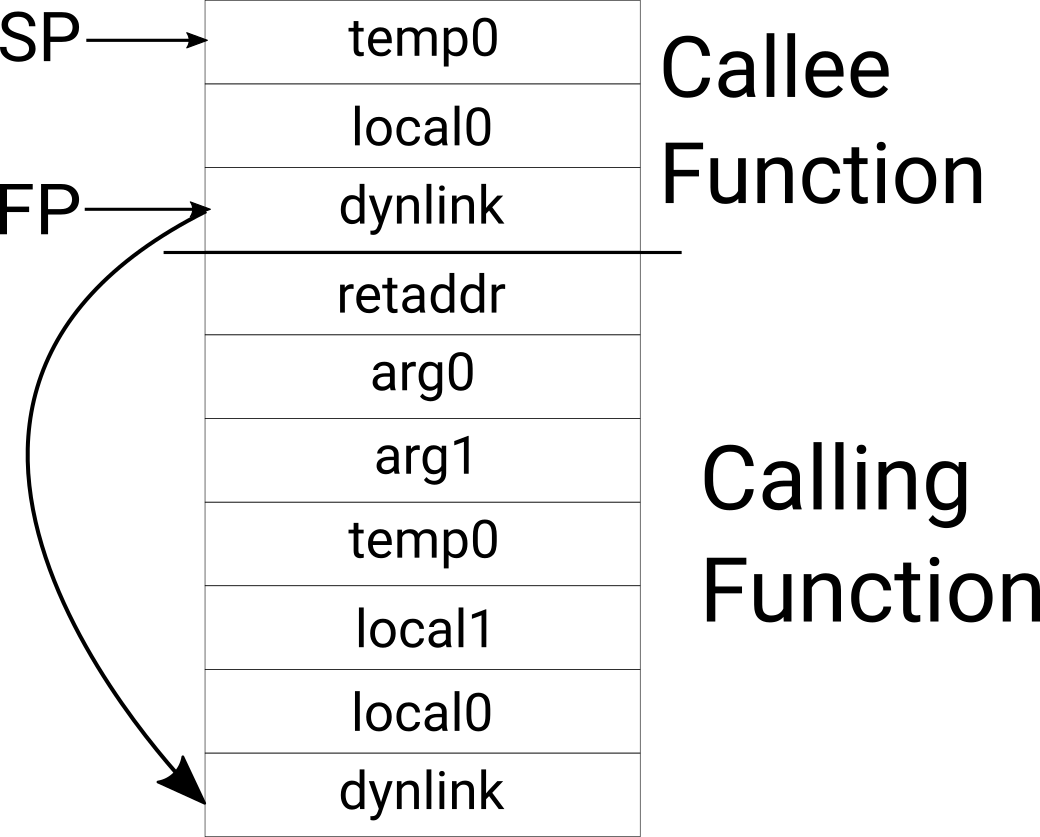
\includegraphics[scale=0.65]{./Stack_Frame.png}
    \caption{Stack Frame}
    \label{fig:Stack_Frame}
  \end{figure}

  Additionally, there are 2 registers used as pointers to move around and interact with the stack frame.
  \begin{enumerate}[noitemsep]
  \item \texttt{FP} is in register \rbpRegister{}. It is the \nameref{def:Frame_Pointer}.
  \item \texttt{SP} is in register \rspRegister{}. It is the \nameref{def:Stack_Pointer}.
  \end{enumerate}
\end{definition}

\begin{definition}[Dynamic Link]\label{def:Dynamic_Link}
  The \emph{dynamic link} or \emph{dynlink} is a memory address pointer and sits at the bottom of a \nameref{def:Stack_Frame}.
  It is a pointer back to the previous function's dynamic link.
  This ensures that any function can find its parent/calling function.

  The dynamic link also serves as a means to access any variable that might be needed by this function.
  To access any variable in \emph{this} function, you can subtract a byte multiple that you need to access the proper value.
  To access any variable in the calling function, you can add a byte multiple that would correspond to the proper variable.

    In the \texttt{x86\textunderscore{} 64} architecture, instruction set, and convention that we used, the register \rbpRegister{} was the dynamic link.
  \begin{remark}
    Note: Due to the conventions we used, when accessing arguments passed to the function, we treated them as local variables, just further down in the call stack.
    This also means that we need to skip over the \nameref{def:Return_Address} block in memory.
  \end{remark}

  \begin{remark}
    Because we used the \rbpRegister{} register to store our current \nameref{def:Dynamic_Link}'s address, the dynamic link might also be called the \emph{base pointer}.
  \end{remark}
\end{definition}

\begin{definition}[Local Variable]\label{def:Local_Variable}
  \emph{Local variables} are handled very simply.
  They get an appropriate amount of memory allocated to them on the stack, and that is it.

  There is no way to give a variable a name in assembly. (Usually. Depends on the architecture and instruction set).
  However, there is no way to name something in memory.
  But, because the size of all the objects is known at compile-time, allocating the proper amount of memory required by each variable is possible.

  \begin{remark}
    This holds true for strongly-typed, static, compiled languages, like Java, C, C++, etc.
    However, Python is slightly different in this regard, and handles it differently.
    That is discussed further in \Cref{subsec:Intermediate_Code}, \nameref{subsec:Intermediate_Code}.
  \end{remark}
\end{definition}

\begin{definition}[Temporary Variable]\label{def:Temporary_Variable}
  A \emph{temporary variable} is one that is allocated on this function's \nameref{def:Stack_Frame} while calculating values.
  Once the calculations are completed, these values are deallocated.
  These temporary variables can also point to objects on the \nameref{def:Heap}.
  When the function has finished running, then these values are deallocated, along with all other \nameref{def:Local_Variable}s in use.

  For example, since assembly-level addition only allows for 2 operands, but in general, addition can have more than 2 operands in use, there needs to be a way to store the value used in the addition.
  While we can accumulate and use that value in the addition, the values being added together are \emph{not} modified.
\end{definition}

\begin{definition}[Static Link]\label{def:Static_Link}
  The \emph{static link} is an implicit argument, meaning it \textbf{\emph{ALWAYS}} gets pushed onto the stack as a \nameref{def:Function_Argument}, when appropriate.

  Appropriate in this context could mean several things:
  \begin{itemize}[noitemsep]
  \item When an object is alive, and when it is being acted on by a function.
    \begin{itemize}[noitemsep]
    \item In this case, the static link points to an instance of a class on the \nameref{def:Heap}.
    \end{itemize}
  \item When a language allows for nested function declarations.
    \begin{itemize}[noitemsep]
    \item Then the static link points to the \nameref{def:Dynamic_Link} of the outer function
    \item This allows access to the outer function's \nameref{def:Local_Variable}s like normal, and allows us to go back later.
    \end{itemize}
  \end{itemize}
\end{definition}

\begin{definition}[Function Argument]\label{def:Function_Argument}
  \emph{Function argument}s are handled very simply.
  If a function call takes an argument, then the argument is calculated, and then that argument is pushed onto the stack in \emph{this} \nameref{def:Stack_Frame}.

  \begin{remark}
    If more than one argument is passed to a function, there are 2 ways to push values onto the \nameref{def:Stack_Frame}:
    \begin{enumerate}[noitemsep]
    \item In the order they are passed to the function
      \begin{itemize}[noitemsep]
      \item Say a function with 3 arguments is called, then the stack would have arguments in this order
        \begin{enumerate}[noitemsep]
        \item argument0 (Lowest memory address)
        \item argument1
        \item argument2 (Highest memory address)
        \end{enumerate}
      \end{itemize}
    \item In reverse order
      \begin{itemize}[noitemsep]
      \item Say the same function is called with the same 3 arguments, then the stack would have arguments in this order
        \begin{enumerate}[noitemsep]
        \item argument2 (Lowest memory address)
        \item argument1
        \item argument0 (Highest memory address)
        \end{enumerate}
      \end{itemize}
    \end{enumerate}
  \end{remark}

  When the values that were passed need to be accessed, and if the memory sizes of things are known at compile time, then we can calculate how far down we need to go in the stack to find the value.
  This is done by adding a positive value to the \rbpRegister{}
\end{definition}

\begin{definition}[Return Address]\label{def:Return_Address}
  The \emph{return address} is used by the \ripRegister{} register.
  It is calculated and pushed onto the \nameref{def:Stack_Frame} stack when the \texttt{CALL} macro is used.
  It is the thing that allows us to jump around in the code from the \texttt{text} area of our program.

  \begin{remark}
    The \ripRegister{} register is the \emph{register instruction pointer}.
    It holds the value of the \emph{next} instruction to execute.
    Technically, it is the Program Counter's value.
  \end{remark}
\end{definition}

\begin{definition}[Garbage Collection]\label{def:Garbage_Collection}
  \emph{Garbage collection} is the act of deallocating objects that may still be on the heap and organizing the heap.
  Since the heap allocates continuous ``blocks'' of memory required by an object, the heap may have the necessary memory to allocate an object, but in discontinuous locations.
\end{definition}

\begin{definition}[Frame Pointer]\label{def:Frame_Pointer}
  The \emph{frame pointer} is a pointer that \textbf{\emph{ALWAYS}} points to the current function's \nameref{def:Dynamic_Link}.
  The frame pointer is commonly abbreviated as \emph{FP}.
  This is the thing that allows us to access \nameref{def:Local_Variable}s, \nameref{def:Function_Argument}s, and everything else inside of the \nameref{def:Stack_Frame}.
  The value is held in the \rbpRegister{} register.
\end{definition}

\begin{definition}[Stack Pointer]\label{def:Stack_Pointer}
  The \emph{stack pointer} is a pointer that \textbf{\emph{ALWAYS}} points to the top of the current \nameref{def:Stack_Frame}.
  The stack pointer is commonly abbreviated as \emph{SP}.
  This value is held in the \rspRegister{} register.
  This is the pointer that allows us to push and pop onto this function's \nameref{def:Stack_Frame}.
\end{definition}

\begin{definition}[Class Descriptor]\label{def:Class_Descriptor}
  The \emph{class descriptor} is a portion of memory set aside for the methods that are in an object.
\end{definition}

\subsection{Making a Function Call}\label{subsec:Making_Function_Call}
There are several steps that must be followed:
\begin{enumerate}[noitemsep]
\item Push the arguments onto the calling function's \nameref{def:Stack_Frame}.
\item Push the \nameref{def:Return_Address}. This is handled by the \texttt{CALL} instruction.
\item Jump to the called method. This is also handled by the \texttt{CALL} instruction.
\item Push the \nameref{def:Frame_Pointer}'s current value onto the Stack.
\item Move the \nameref{def:Stack_Pointer} to the newly pushed \nameref{def:Frame_Pointer}.
\item Run the code for the called function.
\item Put the value to be returned in the \raxRegister{} register
\item Move the \nameref{def:Stack_Pointer} to the \nameref{def:Frame_Pointer} to deallocate all the values on the called function's stack
\item Move the value where the \nameref{def:Frame_Pointer} is into the \nameref{def:Frame_Pointer}, moving the \nameref{def:Frame_Pointer} to the calling function's \nameref{def:Dynamic_Link}.
\item Pop the called function's \nameref{def:Dynamic_Link} off. (The \nameref{def:Stack_Pointer} is pointing to this value).
\item Pop the \nameref{def:Return_Address} off and put the value into the \ripRegister{} register. (The \texttt{RETURN} instruction handles this).
\item Pop the \nameref{def:Function_Argument}s off.
\item Continue the execution of the calling function.
\end{enumerate}

\subsection{What Does the Compiler Compute?}\label{subsec:Compiler_Computation}
The compiler has to compute a couple of things:
\begin{enumerate}[noitemsep]
\item For uses of locals and arguments
  \begin{itemize}[noitemsep]
  \item The offsets to use (Relative to the \nameref{def:Frame_Pointer}).
  \end{itemize}
\item For methods
  \begin{itemize}[noitemsep]
  \item The space needed for \nameref{def:Local_Variable}s and \nameref{def:Function_Argument}s
  \item We typically use \texttt{PUSH} and \texttt{POP} for the allocation and deallocation of variable of \nameref{def:Temporary_Variable}s.
  \end{itemize}
\item If nested methods are supported
  \begin{itemize}[noitemsep]
  \item The number of \nameref{def:Static_Link} levels to use for variable accesses (0 for \nameref{def:Local_Variable}s)
  \item The number of \nameref{def:Static_Link} levels to use for method calls (0 for local methods)
  \end{itemize}
\end{enumerate}

\subsection{Compiler Function Calling Conventions}\label{subsec:Compiler_Function_Call_Conventions}
\begin{itemize}[noitemsep]
\item Caller-save Register: The calling function must save their registers before calling a function
\item Callee-save Register: The called function must save registers that it will use, and restore them before the called function exits.
\item Argument Order: Put \nameref{def:Function_Argument}s onto the calling function's \nameref{def:Stack_Frame} in what order? Forwards or Backwards?
\item Direction: Let the \nameref{def:Call_Stack} grow towards larger or smaller addresses?
\item Allocation of Space for \nameref{def:Local_Variable}s and \nameref{def:Temporary_Variable}s: Push the variables in one big chunk, or push them one at a time?
\end{itemize}

\subsection{Optimizing the Generated Program}\label{subsec:Optimize_Compiler_Program}
There are multiple ways to optimize the assembly program that the compiler generates:
\begin{enumerate}[noitemsep]
\item Store data in registers instead of in memory
  \begin{itemize}[noitemsep]
  \item The return value (Which we are already doing)
  \item As many function arguments as possible
  \item The \nameref{def:Static_Link}
  \item The \nameref{def:Return_Address}
  \end{itemize}
  \begin{itemize}[noitemsep]
  \item If a function call is made, then the registers must not be corrupted
  \end{itemize}
\item Inline some portions of code.
  \begin{itemize}[noitemsep]
  \item Some variable values that are not modified can have their values inlined to later instructions
  \end{itemize}
\end{enumerate}

%%% Local Variables:
%%% mode: latex
%%% TeX-master: "../EDAN65-Compilers-Reference_Sheet"
%%% End:

%====================================APPENDIX====================================
\appendix
\counterwithin{equation}{section}
\counterwithin{definition}{subsection}

% \clearpage
% \subsection{Trigonometry} \label{app:Trig}
	\subsubsection{Trigonometric Formulas} \label{subsubsec:Trig Formulas}
		\begin{equation} \label{eq:Sin plus Sin with diff Angles}
			\sin \left( \alpha \right) + \sin \left( \beta \right) = 2 \sin \left( \frac{\alpha + \beta}{2} \right) \cos\left( \frac{\alpha - \beta}{2} \right)  
		\end{equation}
		\begin{equation} \label{eq:Cosine-Sine Product}
			\cos \left( \theta \right) \sin \left( \theta \right) = \frac{1}{2} \sin \left( 2 \theta \right)
		\end{equation}
	
	\subsubsection{Euler Equivalents of Trigonometric Functions} \label{subsubsec:Euler Equivalents}
		\begin{equation} \label{eq:Euler Sin}
			\sin \left( x \right) = \frac{e^{\imath x} + e^{-\imath x}}{2}
		\end{equation}
		\begin{equation} \label{eq:Euler Cos}
			\cos \left( x \right) = \frac{e^{\imath x} - e^{-\imath x}}{2 \imath}
		\end{equation}
		\begin{equation} \label{eq:Euler Sinh}
			\sinh \left( x \right) = \frac{e^{x} - e^{-x}}{2}
		\end{equation}
		\begin{equation} \label{eq:Euler Cosh}
			\cosh \left( x \right) = \frac{e^{x} + e^{-x}}{2}
		\end{equation}

% \clearpage
% \section{Calculus}\label{app:Calculus}
\subsection{L'Hopital's Rule}\label{subsec:LHopitals_Rule}
L'Hopital's Rule can be used to simplify and solve expressions regarding limits that yield irreconcialable results.
\begin{lemma}[L'Hopital's Rule]\label{lemma:LHopitals_Rule}
  If the equation
  \begin{equation*}
    \lim\limits_{x \rightarrow a} \frac{f(x)}{g(x)} =
    \begin{cases}
      \frac{0}{0} \\
      \frac{\infty}{\infty} \\
    \end{cases}
  \end{equation*}
  then \Cref{eq:LHopitals_Rule} holds.
  \begin{equation}\label{eq:LHopitals_Rule}
    \lim\limits_{x \rightarrow a} \frac{f(x)}{g(x)} = \lim\limits_{x \rightarrow a} \frac{f'(x)}{g'(x)}
  \end{equation}
\end{lemma}

\subsection{Fundamental Theorems of Calculus}\label{subsec:Fundamental Theorem of Calculus}
\begin{definition}[First Fundamental Theorem of Calculus]\label{def:1st Fundamental Theorem of Calculus}
  The \emph{first fundamental theorem of calculus} states that, if $f$ is continuous on the closed interval $\left[ a,b \right]$ and $F$ is the indefinite integral of $f$ on $\left[ a,b \right]$, then

  \begin{equation}\label{eq:1st Fundamental Theorem of Calculus}
    \int_{a}^{b}f \left( x \right) dx = F \left( b \right) - F \left( a \right)
  \end{equation}
\end{definition}

\begin{definition}[Second Fundamental Theorem of Calculus]\label{def:2nd Fundamental Theorem of Calculus}
  The \emph{second fundamental theorem of calculus} holds for $f$ a continuous function on an open interval $I$ and $a$ any point in $I$, and states that if $F$ is defined by

  \begin{equation*}
    F \left( x \right) = \int_{a}^{x} f \left( t \right) dt,
  \end{equation*}
  then
  \begin{equation}\label{eq:2nd Fundamental Theorem of Calculus}
    \begin{aligned}
      \frac{d}{dx} \int_{a}^{x} f \left( t \right) dt &= f \left( x \right) \\
      F' \left( x \right) &= f \left( x \right) \\
    \end{aligned}
  \end{equation}
\end{definition}

\begin{definition}[argmax]\label{def:argmax}
  The arguments to the \emph{argmax} function are to be maximized by using their derivatives.
  You must take the derivative of the function, find critical points, then determine if that critical point is a global maxima.
  This is denoted as
  \begin{equation*}\label{eq:argmax}
    \argmax_{x}
  \end{equation*}
\end{definition}

\subsection{Rules of Calculus}\label{subsec:Rules of Calculus}
\subsubsection{Chain Rule}\label{subsubsec:Chain Rule}
\begin{definition}[Chain Rule]\label{def:Chain Rule}
  The \emph{chain rule} is a way to differentiate a function that has 2 functions multiplied together.

  If
  \begin{equation*}
    f(x) = g(x) \cdot h(x)
  \end{equation*}
  then,
  \begin{equation}\label{eq:Chain Rule}
    \begin{aligned}
      f'(x) &= g'(x) \cdot h(x) + g(x) \cdot h'(x) \\
      \frac{df(x)}{dx} &= \frac{dg(x)}{dx} \cdot g(x) + g(x) \cdot \frac{dh(x)}{dx} \\
    \end{aligned}
  \end{equation}
\end{definition}

\subsection{Useful Integrals}\label{subsec:Useful_Integrals}
\begin{equation}\label{eq:Cosine_Indefinite_Integral}
  \int \cos(x) \; dx = \sin(x)
\end{equation}

\begin{equation}\label{eq:Sine_Indefinite_Integral}
  \int \sin(x) \; dx = -\cos(x)
\end{equation}

\begin{equation}\label{eq:x_Cosine_Indefinite_Integral}
  \int x \cos(x) \; dx = \cos(x) + x \sin(x)
\end{equation}
\Cref{eq:x_Cosine_Indefinite_Integral} simplified with Integration by Parts.

\begin{equation}\label{eq:x_Sine_Indefinite_Integral}
  \int x \sin(x) \; dx = \sin(x) - x \cos(x)
\end{equation}
\Cref{eq:x_Sine_Indefinite_Integral} simplified with Integration by Parts.

\begin{equation}\label{eq:x_Squared_Cosine_Indefinite_Integral}
  \int x^{2} \cos(x) \; dx = 2x \cos(x) + (x^{2} - 2) \sin(x)
\end{equation}
\Cref{eq:x_Squared_Cosine_Indefinite_Integral} simplified by using Integration by Parts twice.

\begin{equation}\label{eq:x_Squared_Sine_Indefinite_Integral}
  \int x^{2} \sin(x) \; dx = 2x \sin(x) - (x^{2} - 2) \cos(x)
\end{equation}
\Cref{eq:x_Squared_Sine_Indefinite_Integral} simplified by using Integration by Parts twice.

\begin{equation}\label{eq:Exponential_Cosine_Indefinite_Integral}
  \int e^{\alpha x} \cos(\beta x) \; dx = \frac{e^{\alpha x} \bigl( \alpha \cos(\beta x) + \beta \sin(\beta x) \bigr)}{\alpha^{2} + \beta^{2}} + C
\end{equation}

\begin{equation}\label{eq:Exponential_Sine_Indefinite_Integral}
  \int e^{\alpha x} \sin(\beta x) \; dx = \frac{e^{\alpha x} \bigl( \alpha \sin(\beta x) - \beta \cos(\beta x) \bigr)}{\alpha^{2}+\beta^{2}} + C
\end{equation}

\begin{equation}\label{eq:Exponential_Indefinite_Integral}
  \int e^{\alpha x} \; dx = \frac{e^{\alpha x}}{\alpha}
\end{equation}

\begin{equation}\label{eq:x_Exponential_Indefinite_Integral}
  \int x e^{\alpha x} \; dx = e^{\alpha x} \left( \frac{x}{\alpha} - \frac{1}{\alpha^{2}} \right)
\end{equation}
\Cref{eq:x_Exponential_Indefinite_Integral} simplified with Integration by Parts.

\begin{equation}\label{eq:Inverse_x_Indefinite_Integral}
  \int \frac{dx}{\alpha + \beta x} = \int \frac{1}{\alpha + \beta x} \; dx = \frac{1}{\beta} \ln (\alpha + \beta x)
\end{equation}

\begin{equation}\label{eq:Inverse_x_Squared_Indefinite_Integral}
  \int \frac{dx}{\alpha^{2} + \beta^{2} x^{2}} = \int \frac{1}{\alpha^{2} + \beta^{2} x^{2}} \; dx = \frac{1}{\alpha \beta} \arctan \left( \frac{\beta x}{\alpha} \right)
\end{equation}

\begin{equation}\label{eq:a_Exponential_Indefinite_Integral}
  \int \alpha^{x} \; dx = \frac{\alpha^{x}}{\ln(\alpha)}
\end{equation}

\begin{equation}\label{eq:a_Exponential_Derivative}
  \frac{d}{dx} \alpha^{x} = \frac{d\alpha^{x}}{dx} = \alpha^{x} \ln(x)
\end{equation}

\subsection{Leibnitz's Rule}\label{subsec:Leibnitzs_Rule}
\begin{lemma}[Leibnitz's Rule]\label{lemma:Leibnitzs_Rule}
  Given
  \begin{equation*}
    g(t) = \int_{a(t)}^{b(t)} f(x, t) \, dx
  \end{equation*}
  with $a(t)$ and $b(t)$ differentiable in $t$ and $\frac{\partial f(x, t)}{\partial t}$ continuous in both $t$ and $x$, then
  \begin{equation}\label{eq:Leibnitzs_Rule}
    \frac{d}{dt} g(t) = \frac{d g(t)}{dt} = \int_{a(t)}^{b(t)} \frac{\partial f(x, t)}{\partial t} \, dx + f \bigl[ b(t), t \bigr] \, \frac{d b(t)}{dt} - f \bigl[ a(t), t \bigr] \, \frac{d a(t)}{dt}
  \end{equation}
\end{lemma}



\clearpage
% To make this print, you must include a citation somewhere in the document
\nocite{CourseTextbook}
\printbibliography{}

\end{document}
%%% Local Variables:
%%% mode: latex
%%% TeX-master: t
%%% End:
